% Options for packages loaded elsewhere
% Options for packages loaded elsewhere
\PassOptionsToPackage{unicode}{hyperref}
\PassOptionsToPackage{hyphens}{url}
\PassOptionsToPackage{dvipsnames,svgnames,x11names}{xcolor}
%
\documentclass[
  11pt,
  a4paper,
]{article}
\usepackage{xcolor}
\usepackage{amsmath,amssymb}
\setcounter{secnumdepth}{-\maxdimen} % remove section numbering
\usepackage{iftex}
\ifPDFTeX
  \usepackage[T1]{fontenc}
  \usepackage[utf8]{inputenc}
  \usepackage{textcomp} % provide euro and other symbols
\else % if luatex or xetex
  \usepackage{unicode-math} % this also loads fontspec
  \defaultfontfeatures{Scale=MatchLowercase}
  \defaultfontfeatures[\rmfamily]{Ligatures=TeX,Scale=1}
\fi
\usepackage{lmodern}
\ifPDFTeX\else
  % xetex/luatex font selection
\fi
% Use upquote if available, for straight quotes in verbatim environments
\IfFileExists{upquote.sty}{\usepackage{upquote}}{}
\IfFileExists{microtype.sty}{% use microtype if available
  \usepackage[]{microtype}
  \UseMicrotypeSet[protrusion]{basicmath} % disable protrusion for tt fonts
}{}
\usepackage{setspace}
\makeatletter
\@ifundefined{KOMAClassName}{% if non-KOMA class
  \IfFileExists{parskip.sty}{%
    \usepackage{parskip}
  }{% else
    \setlength{\parindent}{0pt}
    \setlength{\parskip}{6pt plus 2pt minus 1pt}}
}{% if KOMA class
  \KOMAoptions{parskip=half}}
\makeatother
% Make \paragraph and \subparagraph free-standing
\makeatletter
\ifx\paragraph\undefined\else
  \let\oldparagraph\paragraph
  \renewcommand{\paragraph}{
    \@ifstar
      \xxxParagraphStar
      \xxxParagraphNoStar
  }
  \newcommand{\xxxParagraphStar}[1]{\oldparagraph*{#1}\mbox{}}
  \newcommand{\xxxParagraphNoStar}[1]{\oldparagraph{#1}\mbox{}}
\fi
\ifx\subparagraph\undefined\else
  \let\oldsubparagraph\subparagraph
  \renewcommand{\subparagraph}{
    \@ifstar
      \xxxSubParagraphStar
      \xxxSubParagraphNoStar
  }
  \newcommand{\xxxSubParagraphStar}[1]{\oldsubparagraph*{#1}\mbox{}}
  \newcommand{\xxxSubParagraphNoStar}[1]{\oldsubparagraph{#1}\mbox{}}
\fi
\makeatother


\usepackage{longtable,booktabs,array}
\usepackage{calc} % for calculating minipage widths
% Correct order of tables after \paragraph or \subparagraph
\usepackage{etoolbox}
\makeatletter
\patchcmd\longtable{\par}{\if@noskipsec\mbox{}\fi\par}{}{}
\makeatother
% Allow footnotes in longtable head/foot
\IfFileExists{footnotehyper.sty}{\usepackage{footnotehyper}}{\usepackage{footnote}}
\makesavenoteenv{longtable}
\usepackage{graphicx}
\makeatletter
\newsavebox\pandoc@box
\newcommand*\pandocbounded[1]{% scales image to fit in text height/width
  \sbox\pandoc@box{#1}%
  \Gscale@div\@tempa{\textheight}{\dimexpr\ht\pandoc@box+\dp\pandoc@box\relax}%
  \Gscale@div\@tempb{\linewidth}{\wd\pandoc@box}%
  \ifdim\@tempb\p@<\@tempa\p@\let\@tempa\@tempb\fi% select the smaller of both
  \ifdim\@tempa\p@<\p@\scalebox{\@tempa}{\usebox\pandoc@box}%
  \else\usebox{\pandoc@box}%
  \fi%
}
% Set default figure placement to htbp
\def\fps@figure{htbp}
\makeatother


% definitions for citeproc citations
\NewDocumentCommand\citeproctext{}{}
\NewDocumentCommand\citeproc{mm}{%
  \begingroup\def\citeproctext{#2}\cite{#1}\endgroup}
\makeatletter
 % allow citations to break across lines
 \let\@cite@ofmt\@firstofone
 % avoid brackets around text for \cite:
 \def\@biblabel#1{}
 \def\@cite#1#2{{#1\if@tempswa , #2\fi}}
\makeatother
\newlength{\cslhangindent}
\setlength{\cslhangindent}{1.5em}
\newlength{\csllabelwidth}
\setlength{\csllabelwidth}{3em}
\newenvironment{CSLReferences}[2] % #1 hanging-indent, #2 entry-spacing
 {\begin{list}{}{%
  \setlength{\itemindent}{0pt}
  \setlength{\leftmargin}{0pt}
  \setlength{\parsep}{0pt}
  % turn on hanging indent if param 1 is 1
  \ifodd #1
   \setlength{\leftmargin}{\cslhangindent}
   \setlength{\itemindent}{-1\cslhangindent}
  \fi
  % set entry spacing
  \setlength{\itemsep}{#2\baselineskip}}}
 {\end{list}}
\usepackage{calc}
\newcommand{\CSLBlock}[1]{\hfill\break\parbox[t]{\linewidth}{\strut\ignorespaces#1\strut}}
\newcommand{\CSLLeftMargin}[1]{\parbox[t]{\csllabelwidth}{\strut#1\strut}}
\newcommand{\CSLRightInline}[1]{\parbox[t]{\linewidth - \csllabelwidth}{\strut#1\strut}}
\newcommand{\CSLIndent}[1]{\hspace{\cslhangindent}#1}



\setlength{\emergencystretch}{3em} % prevent overfull lines

\providecommand{\tightlist}{%
  \setlength{\itemsep}{0pt}\setlength{\parskip}{0pt}}



 


\usepackage{fancyhdr}
\usepackage{titling}
\usepackage{graphicx}
\pretitle{\begin{center}\vspace*{1cm}\LARGE\bfseries}
\posttitle{\end{center}}
\pagestyle{fancy}
\fancyhf{}
\fancyhead[L]{\small [Logo Actuarial Cortex]}
\fancyhead[R]{\small\itshape\nouppercase{\leftmark}}
\fancyfoot[C]{\thepage}
\renewcommand{\headrulewidth}{0.4pt}
\makeatletter
\@ifpackageloaded{tcolorbox}{}{\usepackage[skins,breakable]{tcolorbox}}
\@ifpackageloaded{fontawesome5}{}{\usepackage{fontawesome5}}
\definecolor{quarto-callout-color}{HTML}{909090}
\definecolor{quarto-callout-note-color}{HTML}{0758E5}
\definecolor{quarto-callout-important-color}{HTML}{CC1914}
\definecolor{quarto-callout-warning-color}{HTML}{EB9113}
\definecolor{quarto-callout-tip-color}{HTML}{00A047}
\definecolor{quarto-callout-caution-color}{HTML}{FC5300}
\definecolor{quarto-callout-color-frame}{HTML}{acacac}
\definecolor{quarto-callout-note-color-frame}{HTML}{4582ec}
\definecolor{quarto-callout-important-color-frame}{HTML}{d9534f}
\definecolor{quarto-callout-warning-color-frame}{HTML}{f0ad4e}
\definecolor{quarto-callout-tip-color-frame}{HTML}{02b875}
\definecolor{quarto-callout-caution-color-frame}{HTML}{fd7e14}
\makeatother
\makeatletter
\@ifpackageloaded{caption}{}{\usepackage{caption}}
\AtBeginDocument{%
\ifdefined\contentsname
  \renewcommand*\contentsname{Table of contents}
\else
  \newcommand\contentsname{Table of contents}
\fi
\ifdefined\listfigurename
  \renewcommand*\listfigurename{List of Figures}
\else
  \newcommand\listfigurename{List of Figures}
\fi
\ifdefined\listtablename
  \renewcommand*\listtablename{List of Tables}
\else
  \newcommand\listtablename{List of Tables}
\fi
\ifdefined\figurename
  \renewcommand*\figurename{Figure}
\else
  \newcommand\figurename{Figure}
\fi
\ifdefined\tablename
  \renewcommand*\tablename{Table}
\else
  \newcommand\tablename{Table}
\fi
}
\@ifpackageloaded{float}{}{\usepackage{float}}
\floatstyle{ruled}
\@ifundefined{c@chapter}{\newfloat{codelisting}{h}{lop}}{\newfloat{codelisting}{h}{lop}[chapter]}
\floatname{codelisting}{Listing}
\newcommand*\listoflistings{\listof{codelisting}{List of Listings}}
\makeatother
\makeatletter
\makeatother
\makeatletter
\@ifpackageloaded{caption}{}{\usepackage{caption}}
\@ifpackageloaded{subcaption}{}{\usepackage{subcaption}}
\makeatother
\usepackage{bookmark}
\IfFileExists{xurl.sty}{\usepackage{xurl}}{} % add URL line breaks if available
\urlstyle{same}
\hypersetup{
  pdftitle={Propuesta para el desarrollo de una tabla de mortalidad selecta por medio del método de Lee-Carter},
  pdfauthor={Daniel Azuaje},
  pdfkeywords={Lee-Carter, Tabla de mortalidad selecta, datos
censales, Venezuela, R, CSO 1980},
  colorlinks=true,
  linkcolor={blue},
  filecolor={Maroon},
  citecolor={Blue},
  urlcolor={Blue},
  pdfcreator={LaTeX via pandoc}}


\title{Propuesta para el desarrollo de una tabla de mortalidad selecta
por medio del método de Lee-Carter}
\usepackage{etoolbox}
\makeatletter
\providecommand{\subtitle}[1]{% add subtitle to \maketitle
  \apptocmd{\@title}{\par {\large #1 \par}}{}{}
}
\makeatother
\subtitle{Aplicación en R a partir de datos censales y comparación con
la mortalidad observada de una empresa de seguros venezolana}
\author{Daniel Azuaje}
\date{}
\begin{document}
\maketitle
\begin{abstract}
\textbf{Resumen:} El sector asegurador venezolano en seguros de vida,
funerario y afines ha utilizado tablas de mortalidad estáticas (CSO
1958, CSO 1980, Tabla de Mortalidad Venezolana) que en muchos casos
provienen de experiencias ajenas al país o con datos desactualizados. El
artículo 43 de la Ley de la Actividad Aseguradora exige emplear tablas
actualizadas que se adapten a la experiencia de los asegurados. Este
trabajo propone el desarrollo de una tabla de mortalidad selecta
mediante el modelo de Lee-Carter en R, a partir de datos censales (INE
1990, 2001, 2011) y de mortalidad del MPPS (1995-2011), con
reconstrucción poblacional, graduación de tasas y proyección a 2015
(LC15). (Antecedentes.) Se comparan las tasas LC15 con la CSO 1980, con
la mortalidad observada de una aseguradora venezolana y con la Tabla de
Mortalidad Venezolana (2002). (Métodos.) En promedio LC15 queda un 53,8
\% por debajo de la CSO80; la experiencia de la aseguradora está por
debajo de LC15 (esperado por efecto selecto); se obtiene una
aproximación selecta (QxLC15CD) aplicando el porcentaje de diferencia.
(Resultados.) Se recomienda no utilizar la CSO80 por su recargo en tasas
y se sugiere actualizar periódicamente el modelo con datos recientes
para una TDM dinámica venezolana de referencia. (Conclusiones.)

\textbf{Abstract:} The Venezuelan insurance sector for life, funeral and
related lines has relied on static mortality tables (CSO 1958, CSO 1980,
Venezuelan Mortality Table) often based on foreign experience or
outdated data. Article 43 of the Insurance Activity Law requires the use
of updated tables adapted to the experience of the insured. This paper
proposes the development of a select mortality table using the
Lee-Carter model in R, from census data (INE 1990, 2001, 2011) and
mortality data from the Ministry of Health (1995-2011), with population
reconstruction, rate graduation and projection to 2015 (LC15).
(Background.) LC15 rates are compared with CSO 1980, with observed
mortality from a Venezuelan insurer, and with the Venezuelan Mortality
Table (2002). (Methods.) On average LC15 is 53.8\% below CSO80; insurer
experience is below LC15 (expected due to selection); a select
approximation (QxLC15CD) is obtained by applying the difference
percentage. (Results.) Use of CSO80 is not recommended due to its rate
loading, and periodic updating of the model with recent data is
suggested for a Venezuelan dynamic reference table. (Conclusions.)
\end{abstract}


\setstretch{1.5}
\begin{tcolorbox}[enhanced jigsaw, rightrule=.15mm, colbacktitle=quarto-callout-note-color!10!white, colback=white, colframe=quarto-callout-note-color-frame, coltitle=black, breakable, leftrule=.75mm, title={Reproducibilidad}, toprule=.15mm, titlerule=0mm, bottomtitle=1mm, arc=.35mm, toptitle=1mm, opacitybacktitle=0.6, left=2mm, bottomrule=.15mm, opacityback=0]

Los materiales académicos del hub operan bajo una política de datos y
código abiertos. Se requiere que el código fuente (R u otro) y los
conjuntos de datos utilizados estén disponibles en un repositorio
público antes de la publicación. Este manuscrito ha sido vaciado en la
plantilla editorial a partir del Trabajo Final de Pregrado (TFPG) del
autor (tutor: Prof.~Angel Colmenares).

\end{tcolorbox}

\section{Introducción}\label{introducciuxf3n}

\subsection{Contexto y problema}\label{contexto-y-problema}

El trabajo tiene por objeto aportar soluciones al problema que
actualmente tiene el sector asegurador venezolano en el área de seguros
de vida, funerario y afines. El ramo de seguros de vida es considerado
``noble'' a nivel mundial y fue uno de los principales impulsores de las
aseguradoras en Venezuela en décadas pasadas. Se desarrolla un estudio
enfocado en el área técnico-actuarial con especial énfasis en la
mortalidad, con la intención de contribuir al crecimiento del ramo.

El \textbf{planteamiento del problema} se puede resumir en el uso de
\textbf{tablas de mortalidad con datos extranjeros} para la tarificación
de seguros de vida y afines. Una tabla de mortalidad (TDM) puede
interpretarse como un modelo que representa la distribución estadística
del tiempo de supervivencia esperado de los miembros de un grupo
determinado; es la base fundamental para el cálculo de tarifas y
reservas. Las tarifas determinan en gran medida la rentabilidad de la
compañía y el nivel de demanda de los productos; las reservas son los
recursos que las aseguradoras tienen para hacer pagos futuros asociados
a las pólizas vigentes.

En Venezuela, el mercado de productos de vida y afines ha disminuido en
suscripción en los últimos años. Un estudio con las compañías
aseguradoras del mercado (primas 2010-2015) muestra que, aunque las
primas netas cobradas crecen año a año en términos nominales, al aplicar
el índice inflacionario a 2015 (deflactar) el comportamiento real es una
\textbf{disminución importante} en las primas y en la suscripción. Entre
las causas de este fenómeno se encuentran la acelerada inflación, los
planes de incentivos y la \textbf{aplicación de tablas de mortalidad que
no describen el adecuado comportamiento de las probabilidades de muerte
y supervivencia selectas}, muchas de ellas desarrolladas con estudios
ajenos a la población venezolana. Pese a ello, después de deducciones de
gastos administrativos, comisiones y siniestros pagados, el ramo sigue
siendo de utilidad para la mayoría de las aseguradoras, por lo que el
desarrollo de nuevos productos con bases técnicas adecuadas a la
población a asegurar resulta de interés. En la
Table~\ref{tbl-evol-ramos} se presenta la evolución de las primas (sin
deflactar) de los ramos de vida y funerario.

\begin{longtable}[]{@{}
  >{\raggedright\arraybackslash}p{(\linewidth - 8\tabcolsep) * \real{0.0753}}
  >{\raggedright\arraybackslash}p{(\linewidth - 8\tabcolsep) * \real{0.1935}}
  >{\raggedright\arraybackslash}p{(\linewidth - 8\tabcolsep) * \real{0.2258}}
  >{\raggedright\arraybackslash}p{(\linewidth - 8\tabcolsep) * \real{0.2366}}
  >{\raggedright\arraybackslash}p{(\linewidth - 8\tabcolsep) * \real{0.2688}}@{}}
\caption{Evolución de las primas de los ramos de vida y funerario (sin
deflactar). Fuente: SUDEASEG, estudio sectorial
2010-2015.}\label{tbl-evol-ramos}\tabularnewline
\toprule\noalign{}
\begin{minipage}[b]{\linewidth}\raggedright
Año
\end{minipage} & \begin{minipage}[b]{\linewidth}\raggedright
Vida (miles Bs)
\end{minipage} & \begin{minipage}[b]{\linewidth}\raggedright
Crec. \% acum. Vida
\end{minipage} & \begin{minipage}[b]{\linewidth}\raggedright
Funerario (miles Bs)
\end{minipage} & \begin{minipage}[b]{\linewidth}\raggedright
Crec. \% acum. Funerario
\end{minipage} \\
\midrule\noalign{}
\endfirsthead
\toprule\noalign{}
\begin{minipage}[b]{\linewidth}\raggedright
Año
\end{minipage} & \begin{minipage}[b]{\linewidth}\raggedright
Vida (miles Bs)
\end{minipage} & \begin{minipage}[b]{\linewidth}\raggedright
Crec. \% acum. Vida
\end{minipage} & \begin{minipage}[b]{\linewidth}\raggedright
Funerario (miles Bs)
\end{minipage} & \begin{minipage}[b]{\linewidth}\raggedright
Crec. \% acum. Funerario
\end{minipage} \\
\midrule\noalign{}
\endhead
\bottomrule\noalign{}
\endlastfoot
2010 & 878 934 & --- & 441 381 & --- \\
2011 & 913 374 & 3,92 \% & 702 744 & 59 \% \\
2012 & 1 131 544 & 23,89 \% & 627 029 & -11 \% \\
2013 & 1 620 789 & 43,24 \% & 934 843 & 49 \% \\
2014 & 2 336 644 & 44,17 \% & 1 355 495 & 45 \% \\
2015 & 4 056 050 & 73,58 \% & 2 608 075 & 92 \% \\
\end{longtable}

\begin{figure}

\centering{

\pandocbounded{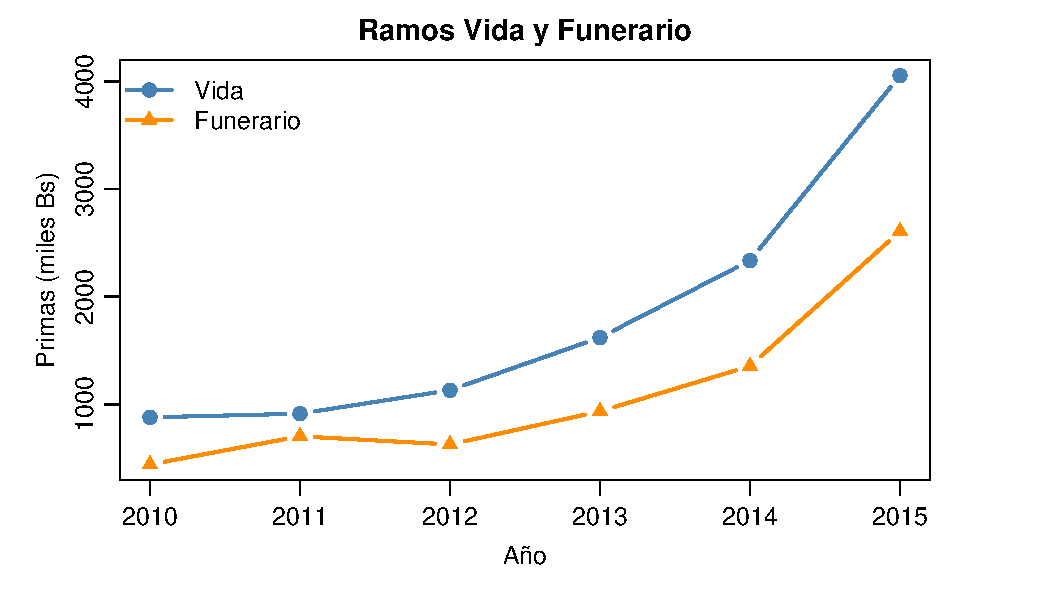
\includegraphics[keepaspectratio]{vol1-azuaje_files/figure-pdf/fig-evol-primas-1.pdf}}

}

\caption{\label{fig-evol-primas}Evolución de las primas (sin deflactar)
de los ramos de vida y funerario, 2010-2015.}

\end{figure}%

\subsection{Marco normativo y tablas en
uso}\label{marco-normativo-y-tablas-en-uso}

El \textbf{artículo 43 (numeral 7)} de la Ley de la Actividad
Aseguradora establece: \emph{``En la elaboración de las tarifas de los
seguros de vida deben emplearse tablas actualizadas de mortalidad o de
supervivencia rentistas, que se adapten en lo posible a la experiencia
de los asegurados de la república''}. La población que integra el
mercado asegurador venezolano tiene características socioeconómicas y
demográficas singulares respecto al resto del país. Tras revisar notas
técnicas presentadas ante la Superintendencia de la Actividad
Aseguradora (SUDEASEG), las tablas de mortalidad \textbf{más utilizadas}
en el sector para beneficios asociados a muerte y supervivencia son las
\textbf{CSO 1958}, \textbf{CSO 1980} y la \textbf{Tabla de Mortalidad
Venezolana} publicada en Gaceta 37429 de abril de 2002. Las tablas CSO
se basan en población estadounidense; la TDM venezolana se desarrolló
con observaciones de 1984 a 1994, comienza a describir la mortalidad
desde los 20 años y en las últimas edades las tasas presentan cambios
bastante radicales. El estudio se enmarca en una de las líneas de
investigación acordadas entre la Escuela de Estadística y Ciencias
Actuariales (EECA-UCV) y la SUDEASEG.

\subsection{Finalidad y objetivos}\label{finalidad-y-objetivos}

\textbf{Finalidad:} Construir una TDM dinámica a partir de los datos de
mortalidad de la población venezolana reportados por el Ministerio del
Poder Popular para la Salud (MPPS) en el periodo 1995-2011, proyectar la
mortalidad hasta 2015 mediante el modelo de Lee-Carter y comparar los
resultados con las TDM usadas por las aseguradoras y con las
estadísticas de defunciones registradas por estas empresas, en
acercamiento a lo exigido por la Ley.

\textbf{Objetivo general:} Propuesta para el desarrollo de una TDM
selecta por medio del modelo de Lee-Carter en lenguaje de programación
R, con datos censales y su comparación con la mortalidad observada de
una empresa de seguros venezolana para el año 2015.

\textbf{Objetivos específicos} (resumidos): conceptualización y
clasificación de tablas de mortalidad; revisión de las TDM realizadas en
Venezuela; evolución de los ramos vida, funerario y afines 2011-2015;
estudio de la metodología para el desarrollo de una TDM; definición y
desarrollo de TDM dinámicas con el método de Lee-Carter; identificación
de fuentes de datos; reconstrucción de la mortalidad poblacional;
proyección de la mortalidad a 2015 en R; comparación de la proyección
con una de las tablas más usadas en el sector; comparación de la TDM
dinámica con la mortalidad observada por una aseguradora venezolana; y
comparación de la dinámica selecta con la Tabla de Mortalidad
Venezolana.

\section{Revisión Literaria}\label{revisiuxf3n-literaria}

\subsection{Tablas de mortalidad
dinámicas}\label{tablas-de-mortalidad-dinuxe1micas}

Las tablas de mortalidad dinámicas o proyectadas son un concepto que
para algunos actuarios en Venezuela puede resultar novedoso, pero a
nivel internacional han tomado gran importancia. Aunque el conocimiento
de la evolución de la mortalidad se remonta a las primeras décadas del
siglo XX, solo recientemente los cálculos actuariales han utilizado
tablas de mortalidad proyectadas o dinámicas; la predicción adecuada de
las probabilidades de muerte mediante este tipo de tablas se ha
convertido en uno de los ejes centrales de la reducción del riesgo
asumido. Predecir con exactitud el proceso de envejecimiento de la
población es una preocupación central en países desarrollados por sus
repercusiones económicas y sociales. En el mismo sentido, el modelo de
dinámica de mortalidad de Lee-Carter ha motivado un cambio en el
análisis de la evolución poblacional, apoyando nuevas hipótesis,
formulaciones y herramientas para generar conclusiones al respecto.

\subsection{Modelo de Lee-Carter}\label{modelo-de-lee-carter}

Las TDM dinámicas no solo toman en cuenta las tasas de mortalidad por
edad sino también las \textbf{generaciones}: la tasa a utilizar depende
de la edad y del año calendario. Existen distintos métodos para su
cálculo; uno de los más recientes y usados en países desarrollados es el
\textbf{método de Lee-Carter (1992)} (Lee \& Carter, 1992). Es un método
paramétrico muy utilizado para tablas dinámicas. Dado un conjunto de
observaciones de tasas en un tiempo específico \(t\) (\(q_{x,t}\)), la
idea principal es obtener a partir de esta muestra una proyección de las
tasas de mortalidad en el tiempo sin cambios bruscos (tasas graduadas).
El modelo es válido para poblaciones no estacionarias, donde las
funciones biométricas dependen de la cohorte \(t\). Lee y Carter
proponen ajustar la medida de la mortalidad en el tiempo así:

\[q_{x,t} = \exp(a_x + b_x k_t + \varepsilon_{xt})\]

o equivalentemente \(\ln(q_{x,t}) = a_x + b_x k_t + \varepsilon_{xt}\),
donde: \(a_x\) es el logaritmo del comportamiento medio de la fuerza de
mortalidad; \(b_x\) describe el patrón de desviación del perfil de edad
\(x\) cuando \(k_t\) varía; \(k_t\) es el \textbf{índice de mortalidad o
tendencia en el tiempo} (define la dirección de la esperanza de vida:
ante una reducción del índice hay mayor esperanza de vida);
\(\varepsilon_{xt}\) es el término de error. En términos de tasas
centrales \(m_{x,t}\) la formulación estándar es
\(\log m_{x,t} = \alpha_x + \beta_x \kappa_t + \epsilon_{x,t}\).

\subsection{Conclusión de la
revisión}\label{conclusiuxf3n-de-la-revisiuxf3n}

La revisión justifica el uso del método Lee-Carter para construir una
tabla dinámica en Venezuela: la bibliografía lo recomienda y muchos
países desarrollados en el área actuarial lo emplean, al permitir
proyectar la mortalidad a futuro con una aproximación cercana a los
datos reales observados.

\section{Métodos}\label{muxe9todos}

\subsection{Fuentes de datos}\label{fuentes-de-datos}

\begin{itemize}
\item
  \textbf{Datos censales:} Desde la página oficial del Instituto
  Nacional de Estadística (INE) se recolectaron los datos censales de
  Venezuela desde 1990 hasta 2011 por grupos de edad de 5 años. Totales
  censados: 1990 (18.105.265), 2001 (23.054.210), 2011 (27.227.930),
  desglosados por sexo (hombres/mujeres).
\item
  \textbf{Mortalidad general:} La información de mortalidad del país se
  extrajo del Ministerio del Poder Popular para la Salud (MPPS):
  registro de muertes desde 1995 a 2011 a nivel nacional, en grupos de
  edades de 5 años y por género, exceptuando la mortalidad infantil que
  se desglosa de forma desagregada.
\item
  \textbf{Aseguradoras:} A partir del Proyecto de unificación de
  solicitudes (SUDEASEG) se obtuvieron expuestos y defunciones de las
  compañías aseguradoras venezolanas para la comparación con la
  mortalidad observada.
\item
  \textbf{Tablas de mortalidad venezolanas históricas:} Se incorporan
  las TDM de Michalub (1941, 1961) y de Luis Escalona (1971) para
  enriquecer la serie temporal en la calibración del Lee-Carter.
\end{itemize}

La Table~\ref{tbl-censos} resume los totales poblacionales de los tres
censos utilizados.

\begin{longtable}[]{@{}llll@{}}
\caption{Total de poblaciones censadas (INE). Fuente: TFPG, Marco
metodológico.}\label{tbl-censos}\tabularnewline
\toprule\noalign{}
Año & Total población & Total hombres & Total mujeres \\
\midrule\noalign{}
\endfirsthead
\toprule\noalign{}
Año & Total población & Total hombres & Total mujeres \\
\midrule\noalign{}
\endhead
\bottomrule\noalign{}
\endlastfoot
1990 & 18 105 265 & 9 019 757 & 9 085 508 \\
2001 & 23 054 210 & 11 402 869 & 11 651 341 \\
2011 & 27 227 930 & 13 549 752 & 13 678 178 \\
\end{longtable}

\subsection{Reconstrucción de la mortalidad
(1995-2011)}\label{reconstrucciuxf3n-de-la-mortalidad-1995-2011}

\begin{enumerate}
\def\labelenumi{\arabic{enumi}.}
\item
  \textbf{Población por sexo:} Se subdividió la población en masculina y
  femenina por censo y por grupos quinquenales de edad. Para el censo
  1990, el grupo ``85 y más'' se desglosó hasta 100 años usando las
  proporciones por edad de CEPAL.
\item
  \textbf{Interpolación entre censos:} Para los años sin censo (entre
  1990, 2001 y 2011) se estimó la población mediante interpolación con
  una función de segundo grado (variable: año; incógnita: cantidad de
  personas en cada grupo de edad).
\item
  \textbf{Edades simples:} Las distribuciones en edades simples se
  tomaron de los censos 2001 y 2011 (INE). Se calculó la proporción de
  personas de cada edad cumplida dentro de cada grupo quinquenal. Para
  1995-2006 se usó la estructura porcentual del censo 2001; para el
  resto de años, la del 2011. Así se distribuyeron tanto la población
  interpolada como las defunciones del MPPS en edades simples por sexo.
\end{enumerate}

\subsection{Cálculo de tasas brutas y
graduación}\label{cuxe1lculo-de-tasas-brutas-y-graduaciuxf3n}

Las \textbf{tasas brutas} de mortalidad (1995-2011 por edad y sexo) se
obtuvieron como cociente entre fallecidos y sobrevivientes para cada
edad. Dado que las proporciones aplicadas generan ``escalones'' en las
gráficas, se \textbf{graduaron} las tasas según la tesis de Ramiro Coa
Clemente mediante el método gráfico: mortalidad infantil con función de
cuarto grado (excepto menores de 1 año); de 5 a 85 años con función
exponencial; de 85 a 100 años por extrapolación exponencial. El
procedimiento se aplicó por género. Con esto se obtuvieron 17 tablas de
mortalidad (una por año) con datos poblacionales venezolanos y tasas
suavizadas.

\subsection{Proyección Lee-Carter en R y tabla
LC15}\label{proyecciuxf3n-lee-carter-en-r-y-tabla-lc15}

El archivo a proyectar contenía las probabilidades de muerte
reconstruidas y graduadas, más las TDM venezolanas (Michalub 1941, 1961;
Escalona 1971) para mejorar la estimación. En \textbf{R} (R Core Team,
2024) se utilizaron las librerías \texttt{demography} (cálculos
Lee-Carter) y \texttt{forecast} (tabla dinámica). Se leyó la data en
formato demográfico (tasas y expuestos por edad, año y sexo) y se ajustó
el modelo Lee-Carter con \texttt{lca()} para las series masculina,
femenina y total hasta edad máxima 100. Los parámetros \(a_x\)
(comportamiento del logaritmo de la fuerza de mortalidad por edad),
\(b_x\) (patrón de desviación cuando \(k_t\) varía) y \(k_t\) (tendencia
en el tiempo) se obtuvieron por serie. La \textbf{proyección} del índice
\(k_t\) se realizó con \texttt{forecast(...,\ h=20)} a 20 años. A partir
de las tasas proyectadas se generó la \textbf{tabla de mortalidad
dinámica} por sexo y total, obteniendo en particular las tasas para el
año \textbf{2015} (LC15). En la Table~\ref{tbl-lc-porcion} se muestra
una porción de la tabla dinámica (probabilidades de muerte \(q_x\) por
edad, años 2012-2016, serie total).

\begin{longtable}[]{@{}llllll@{}}
\caption{Porción de la tabla de mortalidad dinámica por Lee-Carter
(tasas \(q_x\), total). Fuente: TFPG, salida
R.}\label{tbl-lc-porcion}\tabularnewline
\toprule\noalign{}
Edad & 2012 & 2013 & 2014 & 2015 & 2016 \\
\midrule\noalign{}
\endfirsthead
\toprule\noalign{}
Edad & 2012 & 2013 & 2014 & 2015 & 2016 \\
\midrule\noalign{}
\endhead
\bottomrule\noalign{}
\endlastfoot
0 & 0,01728 & 0,01563 & 0,01414 & 0,01280 & 0,01158 \\
1 & 0,00129 & 0,00107 & 0,00089 & 0,00074 & 0,00061 \\
2 & 0,00055 & 0,00045 & 0,00037 & 0,00031 & 0,00025 \\
3 & 0,00038 & 0,00031 & 0,00026 & 0,00021 & 0,00017 \\
4 & 0,00030 & 0,00025 & 0,00021 & 0,00018 & 0,00015 \\
5 & 0,00024 & 0,00020 & 0,00017 & 0,00014 & 0,00012 \\
6 & 0,00030 & 0,00026 & 0,00023 & 0,00019 & 0,00017 \\
7 & 0,00033 & 0,00029 & 0,00026 & 0,00022 & 0,00020 \\
8 & 0,00036 & 0,00032 & 0,00029 & 0,00026 & 0,00023 \\
9 & 0,00040 & 0,00036 & 0,00032 & 0,00029 & 0,00026 \\
10 & 0,00043 & 0,00039 & 0,00036 & 0,00033 & 0,00030 \\
11 & 0,00047 & 0,00043 & 0,00039 & 0,00036 & 0,00033 \\
12 & 0,00050 & 0,00046 & 0,00043 & 0,00040 & 0,00037 \\
13 & 0,00054 & 0,00050 & 0,00046 & 0,00043 & 0,00039 \\
14 & 0,00057 & 0,00053 & 0,00049 & 0,00045 & 0,00042 \\
\end{longtable}

\begin{figure}

\centering{

\pandocbounded{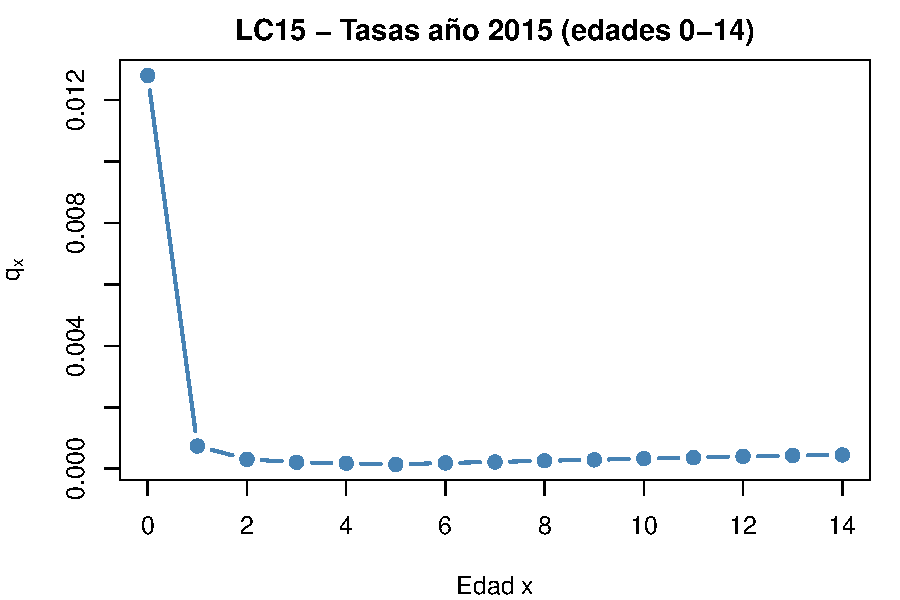
\includegraphics[keepaspectratio]{vol1-azuaje_files/figure-pdf/fig-qx-lc15-edad-1.pdf}}

}

\caption{\label{fig-qx-lc15-edad}Probabilidades de muerte \(q_x\)
proyectadas (LC15) por edad, año 2015 (serie total).}

\end{figure}%

Los parámetros estimados del modelo Lee-Carter (\(a_x\), \(b_x\),
\(k_t\)) se obtienen por serie (masculina, femenina, total). En la
Table~\ref{tbl-param-lc} se muestra una porción de \(a_x\) y \(b_x\)
para la serie total (edades 0-5). El índice \(k_t\) proyectado presenta
tendencia decreciente, coherente con la mejora de la mortalidad en el
tiempo.

\begin{longtable}[]{@{}lll@{}}
\caption{Parámetros Lee-Carter (serie total), edades 0-5. Fuente: TFPG,
salida R (librería demography).}\label{tbl-param-lc}\tabularnewline
\toprule\noalign{}
Edad & \(a_x\) (total) & \(b_x\) (total) \\
\midrule\noalign{}
\endfirsthead
\toprule\noalign{}
Edad & \(a_x\) (total) & \(b_x\) (total) \\
\midrule\noalign{}
\endhead
\bottomrule\noalign{}
\endlastfoot
0 & -3,667 & 0,0135 \\
1 & -5,928 & 0,0250 \\
2 & -6,742 & 0,0264 \\
3 & -7,132 & 0,0259 \\
4 & -7,391 & 0,0243 \\
5 & -7,659 & 0,0237 \\
\end{longtable}

\section{Resultados}\label{resultados}

\subsection{Comparación de la TDM dinámica (LC15) con las tablas más
utilizadas en el
sector}\label{comparaciuxf3n-de-la-tdm-dinuxe1mica-lc15-con-las-tablas-muxe1s-utilizadas-en-el-sector}

Se tomó la mortalidad proyectada a 2015 (LC15) y se comparó con la
\textbf{CSO 1980} (general), una de las tablas más usadas por el sector
asegurador venezolano. La Table~\ref{tbl-lc15-cso80} muestra la
comparación para las primeras edades: la relación porcentual
(LC15/CSO80) indica que \textbf{solo en el primer año de vida} las
probabilidades de LC15 están por encima de la CSO80 (edad 0: 486,63 \%).
En el resto de las edades, las tasas de LC15 están por debajo de la
CSO80. \textbf{En promedio, las tasas de mortalidad de LC15 están un
53,8 \% por debajo de la CSO80.}

\begin{longtable}[]{@{}llll@{}}
\caption{Comparación de tasas \(q_x\) LC2015 y CSO 1980 (porción).
Fuente: TFPG, Análisis de
resultados.}\label{tbl-lc15-cso80}\tabularnewline
\toprule\noalign{}
Edad & CSO80 & LC15 & (LC15/CSO80) \% \\
\midrule\noalign{}
\endfirsthead
\toprule\noalign{}
Edad & CSO80 & LC15 & (LC15/CSO80) \% \\
\midrule\noalign{}
\endhead
\bottomrule\noalign{}
\endlastfoot
0 & 0,00263 & 0,01280 & 486,63 \% \\
1 & 0,00103 & 0,00074 & 71,84 \% \\
2 & 0,00099 & 0,00031 & 30,82 \% \\
3 & 0,00097 & 0,00021 & 21,81 \% \\
4 & 0,00093 & 0,00018 & 19,10 \% \\
5 & 0,00088 & 0,00014 & 15,93 \% \\
\end{longtable}

\begin{figure}

\centering{

\pandocbounded{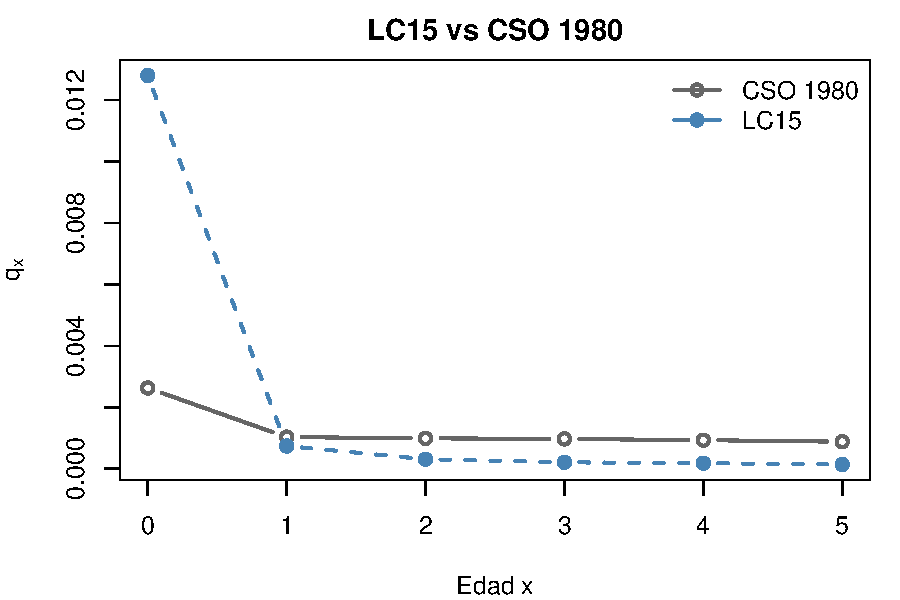
\includegraphics[keepaspectratio]{vol1-azuaje_files/figure-pdf/fig-lc15-cso80-1.pdf}}

}

\caption{\label{fig-lc15-cso80}Comparación de probabilidades de muerte
\(q_x\): LC15 vs CSO 1980 (edades 0-5).}

\end{figure}%

\subsection{Comparación con la mortalidad observada de una aseguradora
venezolana}\label{comparaciuxf3n-con-la-mortalidad-observada-de-una-aseguradora-venezolana}

Se extrajo de los archivos de la SUDEASEG la cartera y siniestros de
vida en 2015 de una de las cinco primeras aseguradoras en el ranking de
primas cobradas del ramo (la muestra no pudo ampliarse por fallas en la
carga de datos). La cartera tiene peso importante en edades 31-60 años,
por lo que el estudio se centró en ese rango. Se calcularon las tasas
brutas a partir de la proporción de siniestros y del número de
expuestos, se suavizaron con el método gráfico (función exponencial) y
se reconstruyó la mortalidad. Al comparar con \textbf{LC2015}, las tasas
de la aseguradora resultaron \textbf{por debajo} de LC15, lo cual era
esperado: LC15 se construye con datos poblacionales (expuestos y muertes
de la población general), mientras que una muestra de asegurados suele
presentar \textbf{efecto selecto} (menor mortalidad). La diferencia
porcentual promedio entre la experiencia de la aseguradora y LC15 fue de
\textbf{14,05 \%} (LC15 por encima). La Table~\ref{tbl-aseg-lc15}
ilustra el cociente Qx(aseguradora)/LC15 para edades 31-35.

\begin{longtable}[]{@{}llll@{}}
\caption{Comparación de LC2015 con la mortalidad observada de una
aseguradora venezolana (porción, edades 31-35). Fuente: TFPG, Análisis
de resultados.}\label{tbl-aseg-lc15}\tabularnewline
\toprule\noalign{}
Edad & Qx Comp. Seg. & LC15 & Qx Comp.Seg / LC15 \\
\midrule\noalign{}
\endfirsthead
\toprule\noalign{}
Edad & Qx Comp. Seg. & LC15 & Qx Comp.Seg / LC15 \\
\midrule\noalign{}
\endhead
\bottomrule\noalign{}
\endlastfoot
31 & 0,00015492 & 0,00135 & 0,1148 \\
32 & 0,00016872 & 0,00145 & 0,1162 \\
33 & 0,00018375 & 0,00156 & 0,1176 \\
34 & 0,00020012 & 0,00168 & 0,1191 \\
35 & 0,00021794 & 0,00181 & 0,1206 \\
\end{longtable}

\begin{figure}

\centering{

\pandocbounded{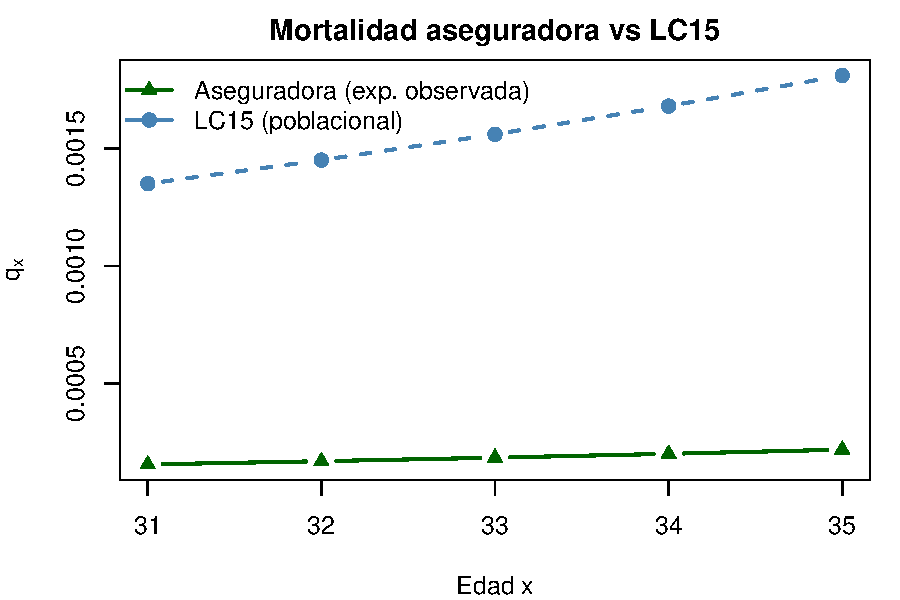
\includegraphics[keepaspectratio]{vol1-azuaje_files/figure-pdf/fig-aseg-lc15-1.pdf}}

}

\caption{\label{fig-aseg-lc15}Tasas \(q_x\) de la aseguradora vs LC15
(edades 31-35). Efecto selecto: experiencia aseguradora por debajo de
LC15.}

\end{figure}%

\subsection{Comparación de la TDM dinámica selecta con la Tabla de
Mortalidad
Venezolana}\label{comparaciuxf3n-de-la-tdm-dinuxe1mica-selecta-con-la-tabla-de-mortalidad-venezolana}

Para aproximar LC15 a un estudio selecto se aplicó un descuento del
14,05 \% a todas las probabilidades de muerte de LC15, obteniendo
\textbf{QxLC15CD} (LC15 con descuento). Esta tabla se comparó con la
\textbf{Tabla de Mortalidad Venezolana} (abril 2002, por sexo). La
Table~\ref{tbl-lc15cd-ven} muestra la relación QxLC15CD con las tasas de
la TDM venezolana para hombres (VEN M) y mujeres (VEN F) en edades
20-27. En el \textbf{caso masculino}, QxLC15CD queda por debajo de la
TDM venezolana en casi todas las edades, excepto en el rango 41-56 años;
en promedio, QxLC15CD representa un \textbf{74,82 \%} de las tasas de la
TDM venezolana de hombres. En el \textbf{caso femenino} hay mayor
similitud; la aproximación selecta de LC15 tiende a estar por debajo
desde la edad 69 hasta el final de la tabla. A nivel práctico, las
aseguradoras en su mayoría no suelen utilizar las tasas femeninas de la
tabla venezolana en las notas técnicas.

\begin{longtable}[]{@{}
  >{\raggedright\arraybackslash}p{(\linewidth - 10\tabcolsep) * \real{0.0741}}
  >{\raggedright\arraybackslash}p{(\linewidth - 10\tabcolsep) * \real{0.2099}}
  >{\raggedright\arraybackslash}p{(\linewidth - 10\tabcolsep) * \real{0.1481}}
  >{\raggedright\arraybackslash}p{(\linewidth - 10\tabcolsep) * \real{0.1481}}
  >{\raggedright\arraybackslash}p{(\linewidth - 10\tabcolsep) * \real{0.2099}}
  >{\raggedright\arraybackslash}p{(\linewidth - 10\tabcolsep) * \real{0.2099}}@{}}
\caption{Comparación de LC15 con descuento (QxLC15CD) y Tabla de
Mortalidad Venezolana (porción, edades 20-27). Fuente: TFPG, Análisis de
resultados.}\label{tbl-lc15cd-ven}\tabularnewline
\toprule\noalign{}
\begin{minipage}[b]{\linewidth}\raggedright
Edad
\end{minipage} & \begin{minipage}[b]{\linewidth}\raggedright
Qx LC15 (desc.)
\end{minipage} & \begin{minipage}[b]{\linewidth}\raggedright
Qx VEN (M)
\end{minipage} & \begin{minipage}[b]{\linewidth}\raggedright
Qx VEN (F)
\end{minipage} & \begin{minipage}[b]{\linewidth}\raggedright
QxLC15CD/VEN(M)
\end{minipage} & \begin{minipage}[b]{\linewidth}\raggedright
QxLC15CD/VEN(F)
\end{minipage} \\
\midrule\noalign{}
\endfirsthead
\toprule\noalign{}
\begin{minipage}[b]{\linewidth}\raggedright
Edad
\end{minipage} & \begin{minipage}[b]{\linewidth}\raggedright
Qx LC15 (desc.)
\end{minipage} & \begin{minipage}[b]{\linewidth}\raggedright
Qx VEN (M)
\end{minipage} & \begin{minipage}[b]{\linewidth}\raggedright
Qx VEN (F)
\end{minipage} & \begin{minipage}[b]{\linewidth}\raggedright
QxLC15CD/VEN(M)
\end{minipage} & \begin{minipage}[b]{\linewidth}\raggedright
QxLC15CD/VEN(F)
\end{minipage} \\
\midrule\noalign{}
\endhead
\bottomrule\noalign{}
\endlastfoot
20 & 0,000537 & 0,00091 & 0,00021 & 0,59 & 2,56 \\
21 & 0,000570 & 0,00093 & 0,00023 & 0,61 & 2,48 \\
22 & 0,000607 & 0,00095 & 0,00025 & 0,64 & 2,43 \\
23 & 0,000649 & 0,00097 & 0,00028 & 0,67 & 2,32 \\
24 & 0,000696 & 0,00100 & 0,00031 & 0,70 & 2,24 \\
25 & 0,000747 & 0,00103 & 0,00034 & 0,73 & 2,20 \\
26 & 0,000804 & 0,00106 & 0,00038 & 0,76 & 2,12 \\
27 & 0,000865 & 0,00109 & 0,00041 & 0,79 & 2,11 \\
\end{longtable}

\begin{figure}

\centering{

\pandocbounded{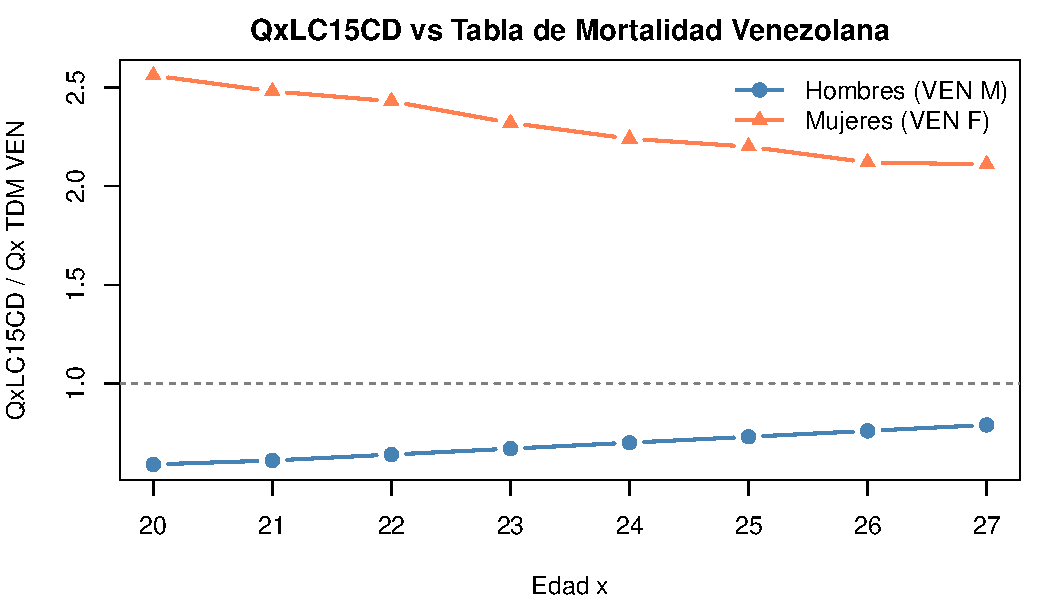
\includegraphics[keepaspectratio]{vol1-azuaje_files/figure-pdf/fig-lc15cd-ven-1.pdf}}

}

\caption{\label{fig-lc15cd-ven}Relación QxLC15CD / TDM Venezolana por
sexo (edades 20-27). Valores \textless{} 1 indican QxLC15CD por debajo
de la TDM VEN.}

\end{figure}%

\section{Discusión y Conclusiones}\label{discusiuxf3n-y-conclusiones}

\subsection{Síntesis de hallazgos}\label{suxedntesis-de-hallazgos}

Se realizó la conceptualización de una tabla de mortalidad y su
clasificación, el repaso de las TDM elaboradas en Venezuela en las
últimas décadas y el análisis de la evolución de los ramos funerario,
vida y afines (2011-2015), que evidencia una situación preocupante: el
cobro de primas en términos reales ha disminuido notablemente. Se
revisaron los métodos para el desarrollo de una TDM y se definieron las
tablas de mortalidad dinámicas con énfasis en el método de Lee-Carter.
Se recopiló información censal del INE, aproximaciones poblacionales de
CEPAL, defunciones del MPPS y las TDM históricas venezolanas del
Ministerio de Fomento. Se recomienda que las instituciones públicas
realicen estudios de esta magnitud con mayor frecuencia y dispongan de
una biblioteca virtual para consultar el histórico de datos.

\subsection{Recomendaciones técnicas}\label{recomendaciones-tuxe9cnicas}

\begin{itemize}
\item
  \textbf{No utilizar la tabla CSO80} para tarificación en Venezuela:
  tiene un recargo en las tasas que se traduce en primas más altas en
  los ramos de vida y funerario; la proyección LC15 muestra en promedio
  tasas 53,8 \% por debajo de la CSO80.
\item
  \textbf{Actualizar periódicamente} el código del modelo Lee-Carter con
  datos más recientes para dar seguimiento a la evolución de las tasas
  de mortalidad.
\item
  \textbf{Carga de datos de aseguradoras:} Solo se logró data completa
  de una aseguradora para las comparaciones; se sugiere a las compañías
  una mejor supervisión de carga y procesamiento de datos de asegurados
  para contar con muestras más óptimas en futuros estudios.
\item
  \textbf{Tabla selecta propuesta:} La diferencia porcentual entre la
  experiencia de la aseguradora y LC15 (14,05 \%) se aplicó sobre la
  proyección LC15 para obtener la tabla selecta (QxLC15CD) que se
  propone en el estudio. Con una muestra más robusta de asegurados y
  siniestros, se recomienda una nueva comparación con la proyección
  Lee-Carter para establecer de forma definitiva una nueva TDM dinámica
  venezolana para el sector asegurador.
\end{itemize}

\subsection{Responsabilidad del
sector}\label{responsabilidad-del-sector}

Es responsabilidad de quienes desempeñan labores en este mercado dar
propuestas y soluciones para mejorarlo, en especial en el área
técnico-actuarial. Las herramientas utilizadas como base para las notas
técnicas del ramo están bastante desfasadas: la CSO80 se basa en datos
estadounidenses y tiene más de 30 años desde su desarrollo; la Tabla
Venezolana se construyó con población selecta 1984-1994. Una
actualización de datos sería de gran utilidad para la industria y el
regulador (SUDEASEG).

\section*{Agradecimientos}\label{agradecimientos}
\addcontentsline{toc}{section}{Agradecimientos}

Agradecimiento al \textbf{Prof.~Angel Colmenares}, tutor del TFPG, por
su orientación y apoyo durante el desarrollo de la investigación; al
jurado evaluador, a la Escuela de Estadística y Ciencias Actuariales
(EECA-UCV) y a Actuarial Cortex por el apoyo en la formación y en la
difusión de este trabajo.

\section*{Referencias}\label{referencias}
\addcontentsline{toc}{section}{Referencias}

La lista de referencias se generará automáticamente a partir del archivo
\texttt{references.bib} y las citas en el texto. Incluir, entre otras, a
Lee y Carter (1992) y a las fuentes citadas en la revisión literaria y
en métodos.

\phantomsection\label{refs}
\begin{CSLReferences}{1}{0}
\bibitem[\citeproctext]{ref-lee1992}
Lee, R. D., \& Carter, L. R. (1992). Modeling and forecasting u.s.
mortality. \emph{Journal of the American Statistical Association},
\emph{87}(419), 659--671.
\url{https://doi.org/10.1080/01621459.1992.10475265}

\bibitem[\citeproctext]{ref-Rcore}
R Core Team. (2024). \emph{R: A language and environment for statistical
computing}. R Foundation for Statistical Computing.
\url{https://www.R-project.org/}

\end{CSLReferences}




\end{document}
